\documentclass{beamer}
\usetheme{metropolis}           % Use metropolis theme
\title{Individual-based modelling of COVID-19 on the Acadia University campus with a realistic contact structure}
\date{August 12, 2020}
\author{\footnotesize Acadia Covid-19 Modelling Group: D. Currie, C. Hooper, M. Hopkins,\linebreak  R. Karsten, Y. Li, F. Mendivil,  H. Teismann}
\institute{AARMS COVID-19 Seminar}
\begin{document}
  \maketitle
  \section*{Introduction}
  \begin{frame}{Introduction: Acadia's Fall 2020 plan (``hybrid'' model) }
 \begin{itemize}
   \item Cap on in-person classes \pause 
   \item Instruction partially online \pause
   \item Risk-reducing behaviour enforced\pause 
   \item Ready to ``pivot'' \pause 
   \item etc. pp.   
\end{itemize}
\end{frame}
 \begin{frame}{Introduction: Similar work}
 \begin{itemize}
 \item Gressman \& Peck \cite{gressman2020simulating}\pause 
 \item Pennsylvania schools {\tiny \href{https://ies.ed.gov/ncee/edlabs/regions/midatlantic/pdf/ReopeningPASchools.pdf}{https://ies.ed.gov/ncee/edlabs/regions/midatlantic/pdf/ReopeningPASchools.pdf} }\pause 
 \item etc. pp 
 \end{itemize}
 \end{frame}
  \section*{Model description}
  \begin{frame}{Model description: Principles (Markov-chain model)}
 \begin{itemize}
  \item[] \textit{discrete time} (denoted by the letter $t$ below; we used  ``day'' as the time increment) \pause 
  \item[] \textit{individual-based}. state  vector $y(t)\in \{0,\ldots ,8\} ^{N_{pop}}$, where  $N_{pop} =$ size of population and $0,1,\ldots ,8$ = stages of disease. \pause 
  \begin{center}
  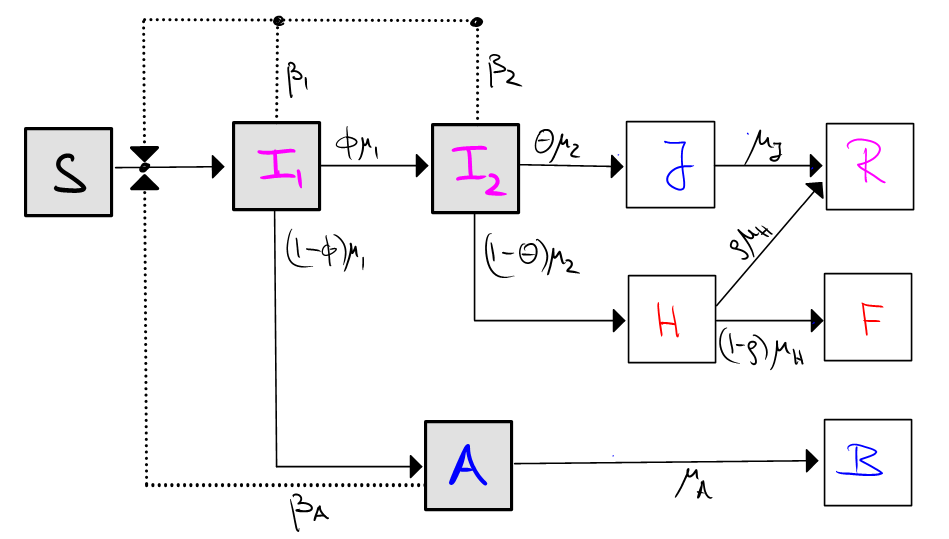
\includegraphics[scale=0.38]{SIIAR-diagram-AARMS-1.png} 
  \end{center}  
\end{itemize}
\end{frame}
\begin{frame}{Model description: Principles (Markov-chain model)}
\textit{stochastic}. in each time step $t\to t+1$ the state vector transitions stochastically  between states according to the transition  matrix {\tiny 
   \[ \left. \begin{array}{c|ccccccccc}
   & S & E+I_1 & I_2 & A & J & H & R & F & B \\
  \hline 
S & 1-b& b& 0 & 0 & 0 & 0 & 0 & 0 & 0 \\
   E+I_1 &0 & 1-\mu _1 & \phi \mu _1 & (1-\phi)\mu _1 & 0 & 0 & 0 & 0 & 0 \\
 I_2 & 0 & 0 & 1-\mu _2 & 0 &\theta \mu _2 & (1-\theta )\mu _2 & 0 & 0 & 0   \\
  A & 0 & 0 & 0 &  1-\mu _A  & 0 & 0 & 0 & 0  & \mu _A   \\
   J &  0 & 0 & 0 & 0 & 1-\mu _J  & 0 & \mu _J & 0  & 0   \\
    H &  0 & 0 & 0 & 0 & 0  & 1-\mu _H & \rho \mu _H & (1-\rho )\mu _H  & 0  \\
     R &  0 & 0 & 0 & 0 & 0  & 0 & 1 & 0  & 0   \\
       F &  0 & 0 & 0 & 0 & 0  & 0 & 0 & 1  & 0   \\
         B &  0 & 0 & 0 & 0 & 0  & 0 & 0 & 0  & 1   \\
   \end{array} \right. \]  } \pause 
{\tiny  where 
\begin{align*}   
 b &= 1- \prod_{j'=1}^{N_{pop}} \Big(1-  \beta (x_{j'}(t),y_{j'}(t))\Big)^{C_{j,j'}} \qquad \textrm{(probability that individual $j$ gets infected)} \\
 C_{j,j'} &= \parbox[t]{14cm}{ contact matrix (average number of infectious contacts between  individuals $j$ and $j'$ per day)}\\
 \beta (x,y) & = \left\{ \begin{array}{cl} \beta _1(x) , & \textrm{if } y = 1 \\
 \beta _2(x) , & \textrm{if } y = 2 \\
 \beta _A(x) , & \textrm{if } y  = 3 \\
 0 , & \textrm{otherwise}
\end{array} \right.   \qquad \qquad \textrm{(probability of infection per contact)} \\
 x_{j}(t) &=  \textrm{infection age (time since individual $j$ got infected)} \\
  %\\   & = t- \inf \{ 0\le s< t \mid y_j(s+1) -y_j(s) >0\}  \\ 
 \mu _*  &= \mu _* (x_j(t)) %\quad \nu \in \{ 1,2,A,J,H\}  
 \quad \parbox[t]{10cm}{(probability of advancing to  next stage of disease )} 
 \\ \phi ,\theta ,\rho & =  \quad \textrm{probabilities of branching.}
\end{align*} }
  \end{frame}
  \begin{frame}{Model description: Parameters}
  \begin{itemize}
 \item We choose $\beta _1(x) \equiv  \beta _2(x) \equiv \beta _A(x) \equiv \beta b(x)$, where  
  the function $b(x) $ is expected to follow the temporal shape of ``viral shedding'' \cite{he2020temporal,ali2020serial,van2020shedding}:
 \begin{center}
 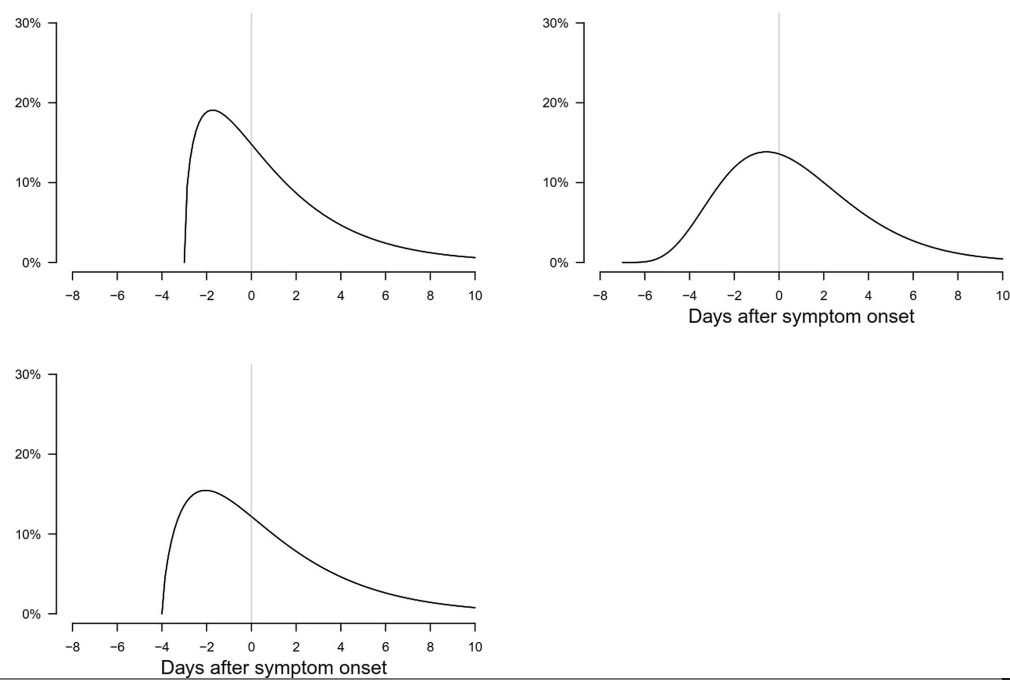
\includegraphics[scale=0.25]{infprofiles.png}  
 \end{center}
 \end{itemize} 
  \end{frame}
    \begin{frame}{Model description: Parameters}
  \begin{itemize}
  \item Similarly, the functions $\mu  _\nu (x)$ have a general shape like this: 
 \begin{center}
 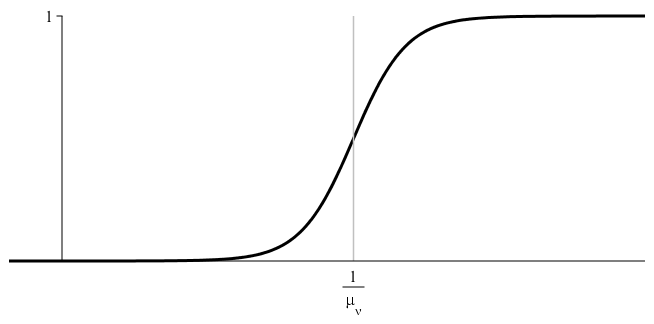
\includegraphics[width=5cm,height=2.3cm]{mushape.png} 
 \end{center} 
 \item The probability of infection per contact  $\beta $ is chosen such that $\mathcal{R}_0
 \approx 3.8$ (value chosen in \cite{gressman2020simulating}).    Here ``contact'' is interpreted as ``being in the same
 room for 15 mins.'' 
 \item  The (median) times $\frac{1}{\mu _\nu}$ in the various stages are typical values found in the literature; see e.g. \cite{ferretti2020quantifying,Ferretti2020.03.08.20032946,ferguson2020report,russell2020using,prem2020wuhan}, \href{https://gabgoh.github.io/COVID/index.html}{https://gabgoh.github.io/COVID/index.html}
 %We chose \\
 %\begin{tabular}{} 
 
\end{itemize} 
  \end{frame}
  
    \begin{frame}{Model description: Parameters}
  \begin{itemize}
  \item Summary (ignoring hospitalizations and deaths for now):  
  \begin{center}
  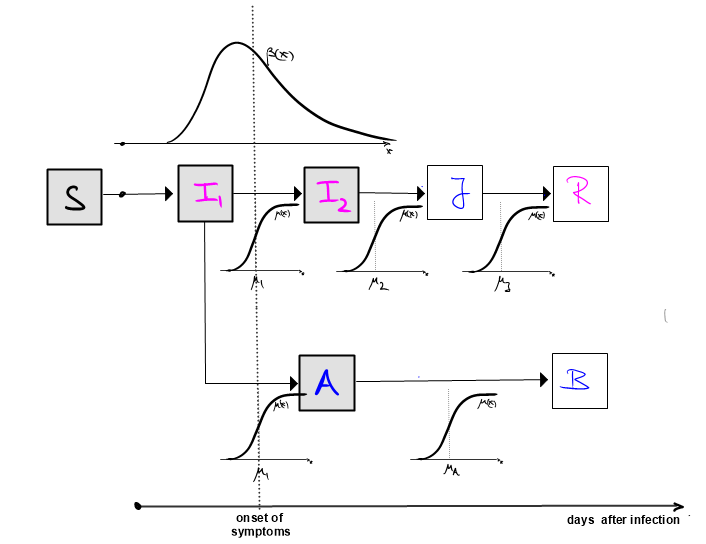
\includegraphics[scale=0.45]{SIIAR-diagram-AARMS-2.png} 
  \end{center}  
\end{itemize} 
  \end{frame}

  
  \begin{frame}{Model description: reproduction number and serial interval}
   \begin{itemize}
 \item \cite{he2020temporal} has this pedagogical diagram:  
 \begin{center}
  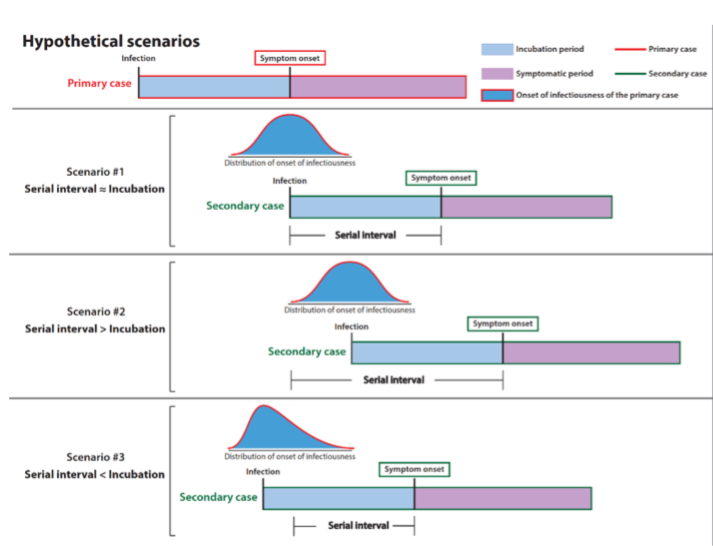
\includegraphics[scale=0.32]{Leung.png} 
 \end{center}
 \end{itemize} 
  \end{frame}
  
  \section*{Contact structure}
   \begin{frame}{Contact structure: Classes}
  \end{frame}
   \begin{frame}{Contact structure: Residences}
  \end{frame}
   \begin{frame}{Contact structure: Off-campus living}
  \end{frame}
   \begin{frame}{Contact structure: Social life}
  \end{frame}
  \section*{Simulation results}
   \begin{frame}{Results: baseline (regular semester, no intervention)}
  \end{frame}
   \begin{frame}{Results: quarantining index cases and contacts}
  \end{frame}
  \begin{frame}{Results: add campus lockdown ...}
  \end{frame}
  \begin{frame}{Results: testing protocol 1}
  \end{frame} 
   \begin{frame}{Results: testing protocol 2}
  \end{frame} 
   \begin{frame}{Results: ``onboarding''}
  \end{frame} 
  \section*{Outlook}
  \begin{frame}{Outlook}
  \begin{itemize}
  \item Study different ``onboarding'' protocols (number and timing of tests etc)   \pause 
  \item Estimate risk of case importation during semester \pause 
  \item Study effects of time delays \pause 
  \item Study effects of compliance \pause
  \item Estimate risk of need to ``pivot'' \pause
  \item etc. pp    
  \end{itemize} 
  \end{frame} 
   \begin{frame}[allowframebreaks]{References}
   \bibliography{Bib}
\bibliographystyle{amsplain} 
  \end{frame} 
\end{document}
